\documentclass[]{usiinfbachelorproject}

\usepackage{color}
\usepackage{caption}
\usepackage{subcaption}

\captionsetup{labelfont={bf}}

\author{Robert Jans}

\title{Experimental Apparatus \\ for a Digital Health Literacy Experiment}
\subtitle{(DRAFT)}
\versiondate{\today}

\begin{committee}
%With more than 1 advisor an error is raised...: only 1 advisor is allowed!
\advisor[Universit\`a della Svizzera Italiana, Switzerland]{Prof.}{Marc}{Langheinrich}
%You can comment out  these lines if you don't have any assistant
\assistant[Universit\`a della Svizzera Italiana, Switzerland]{Prof.}{Peter}{Schulz}
%\assistant[Universit\`a della Svizzera Italiana, Switzerland]{Title}{AssistantName2}{AssistanSurname2}
\end{committee}

\abstract {

    In this project we implement an software toolkit needed for an experiment planned by the \newline
    \emph{Institute~of~Communication~and~Health (ICH)}. The institute is part of the \emph{Faculty of Communication Sciences}
    at the \emph{Università della Sizzera Italiana}. Health communication is a relatively new and multidisciplinary field, 
    which includes the study and use of communication to inform and affect decision making at the individual and community 
    level in order to improve the quality of healthcare \cite{ICH_web}. 
    The purpose of the planned experiment is to investigate the digital health literacy of participants in the
    area of sleeping disorders.
    
    This project seeks to provide the experimental apparatus which will allow the research team to record data an test its hypoteses.
    The project's main tasks are indexing a predefined set of websites, creating a user interface similar to common search engines that
    can be configured to selectively show different subsets of the corpus according to the experimental conditions under inestigation
    and setting up an experimental environment allowing to conduct controlled experimments (e.g. prevent participants from
    accessing non-corpus sites) and to record salient data such as search logs and click-stream.
}


\begin{document}
\maketitle

%%%%%%%%%%%%%%%%%%%%%%%%%
\section{Introduction} \label{introduction}
%%%%%%%%%%%%%%%%%%%%%%%%%

\subsection{Motivation}

Since the beginning of modern science researchers needed special tools in order to conduct experiments. These tools consist 
mainly in devices for taking measurements and triggering phenomena under controlled conditions. Whereas in the past the
experimental apparatuses comprised almost exclusively physical devices, nowadays increasingly more software is involved.
The experiment for which the result of my project is going to be used is a case in which the process of 
setting up the experimental conditions an collecting the result data depends heavily on the software toolkit. It is therefore
essential for the software to be robust and reliable.

My personal motivations Come from two sides: I have a general interest in science an the scientific method, but in practice,
rather than as a scientist,
I see myself as a technician, who in the area of of software development seeks to build useful applications.
Int that sense this project perfectly fits my interests, as it involves the creation of software to be used in the context of
scientific research.    

\subsection{Outline}
\TODO{}


%%%%%%%%%%%%%%%%%%%%%%%%%
\section{Requirements} \label{requirements}
%%%%%%%%%%%%%%%%%%%%%%%%%

Below is a description of the requirements as defined by the advisor. The requirements include three main tasks as well 
as eight milestones; the milestones are divided into the categories \emph{Must have}, \emph{should have}, and \emph{Nice to have}.

\subsection{Main Tasks}
    \begin{enumerate}

        \item Spidering (i.e. creating a full or partial local copy of) a predefined set of websites that provide
              sleeping disorder information as an experimental corpus. 

        \item Creating a Google-like search interface to the corpus that can be configured to selectively show/rank different sets of
              corpus sites, according to the experimental conditions under investigation.

        \item Setting up an experimental environment (e.g. using the \emph{SafeExamBrowser}, or using a proxy server) to
              conduct controlled experiments using the corpus (e.g. to prevent participants from accessing non-corpus sites)
              and to record salient data (e.g. search logs, click-stream).

    \end{enumerate} 

\subsection{Milestones}
    \begin{enumerate}

        \item \textbf{(Must have)} A website which simulates a search engine that lets users enter keywords into a search form and
              returns results (snippets) from a predefined corpus of websites/links, which can then be clicked on / followed.

        \item \textbf{(Must have)} A result generator and a simple way to configure it (e.g. using a text file) on a per-group
              basis (i.e. participants in Group 1 receive result from lists R1, R2, and R3; Group 2 participants
              receive results from R4, R2 and R3).

        \item \textbf{(Must have)} A report describing the system setup/installation and the architectural design. 

        \item \textbf{(Should have)} A result generator that can detect identical, repeated queries (or minor variations of
              otherwise identical queries, detectable via stop word removal and stemming) upon which it will generate the same response.

        \item \textbf{(Should have)} A detailed log engine which allows the experimenter to track key experimental results
              for each participant, such as search terms entered, the time spent on a given result list and any clicks on
              results (when, which order).

        \item \textbf{(Should have)} A visual presentation of the search entry and result section that mimics a known search engine.  

        \item \textbf{(Nice to have)} A result generator that can handle non-related searches using a pass-through to a real search engine.

        \item \textbf{(Nice to have)} A web interface to the log engine that allows for convenient inspection, analysis,
              and export of experimental results.

    \end{enumerate}

%%%%%%%%%%%%%%%%%%%%%%%%%
\section{Project design} \label{design}
%%%%%%%%%%%%%%%%%%%%%%%%%

\subsection{General architecture}

Given the close relationships between the experiment configuration, conduction, and analysis, I decided to include
most of the implied functionalities into a single web application, called \emph{HSE (Health Search Engine)}.
The user management functionality of HSE allows participants to access only a search interface, while experimenters
have access to pages for managing corpora and experiments. If needed, participants can be prevented from
accessing non-corpus sites by restricting the browser to a whitelist based on the corpus used for a given experiment.
The following subsections briefly describe the usage modalities and the related user interfaces.

\subsection{Typical usage workflow}

The typical workflow includes four steps: preparing the document corpora, setting up an experiment, running the experiment
and finally evaluating the resulting data. \textbf{Figure ~\ref{fig:usage}} shows this usage scenario. 
To each usage step corresponds a dedicated user interface. 

For preparing the corpora the experimenter provides text files containing the web URL's of the chosen documents. After setting the names for the
corresponding document collection, the application takes care of downloading the contents and creating the inverted indices needed for retrieval.
Setting up an experiment involves defining test groups and assigning participants to each group. Moreover for each test group it is needed
to set the document collections from which the retrieval mechanism will select the results to be displayed to the participants.
The groups cab be defined either manually or by uploading a configuration file.
The U.I. for experiment execution includes a control button for starting, stopping, or resetting an experiment, as well 
as a tabular display for real time monitoring, showing the current number of queries and clicks for each participant.
Starting an experiment enables the participants tos log in, and initiates the data collection mechanism; after
stopping the experiment, the participants are logged out, and transient data is saved.
The experiment evaluation interface  allows for quick inspection through data summaries and visualizations. Moreover it allows
to export both the raw data and the summaries as files.

\vspace{1cm}

\begin{figure} [h]
\centering
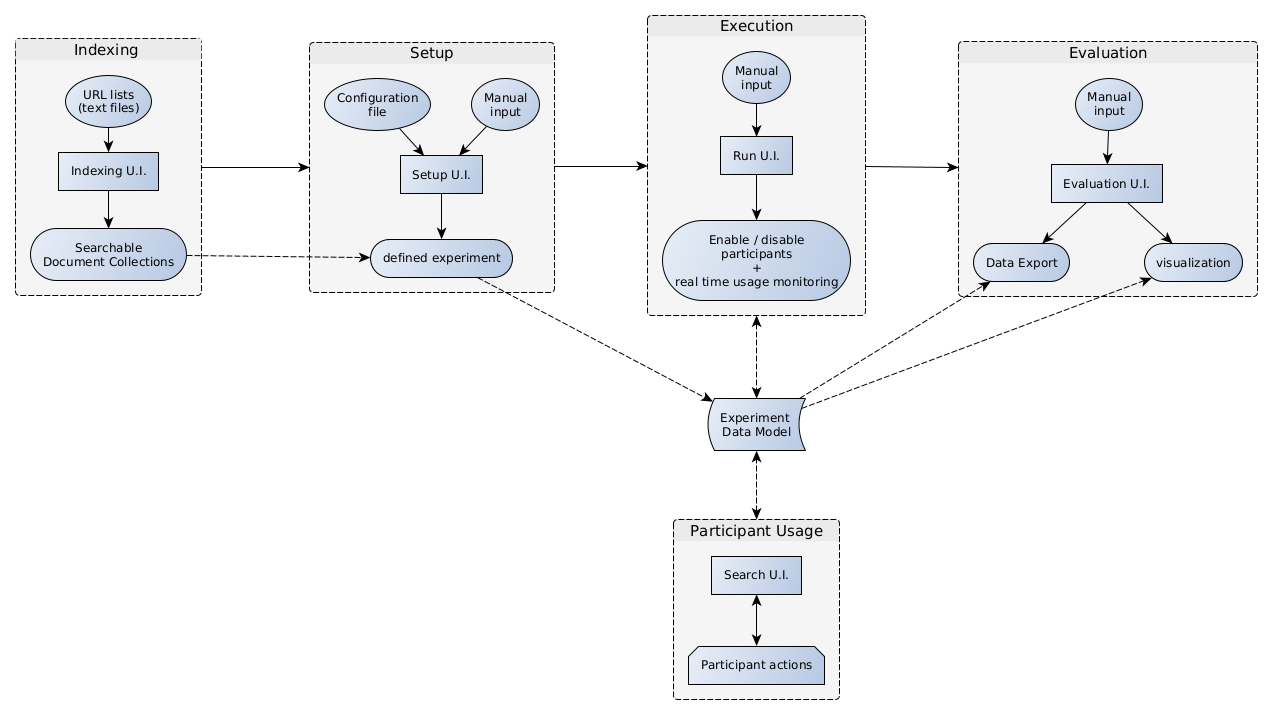
\includegraphics[width=0.8\textwidth]{img/yed/usage}
\caption{Typical usage workflow}
\label{fig:usage}
\end{figure}


\newpage

\subsection{Defining the document corpora}

In order to define the document collections (corpora) to be used during subsequent experiments, 
an experimenter can upload text files containing lists of web URL's. The files are  stored, so they can be reused 
for defining multiple document collections. Via a popup menu a new  document collection can be defined by providing a name, 
the collection's language the related url list.
Clicking on the ''index'' button initiates the indexing process, which includes data download and the creation of a index
data structure for retrieval. The details of the indexing process are explained in section xxx \TODO{link actual section}.
\textbf{Figures ~\ref{fig:indexingA} and ~\ref{fig:indexingB}} show the relevant parts of the interface.

\begin{figure}[h]
     
     \centering
     \begin{subfigure}[b]{0.6\textwidth}
         \centering
         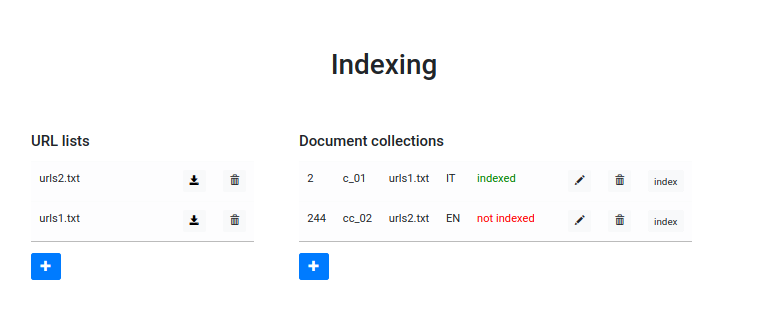
\includegraphics[width=.8\linewidth]{img/indexing1}
         \caption{indexing  u.i}
         \label{fig:indexingA}
     \end{subfigure}
  %   \hfill
     \begin{subfigure}[b]{0.3\textwidth}
         \centering
         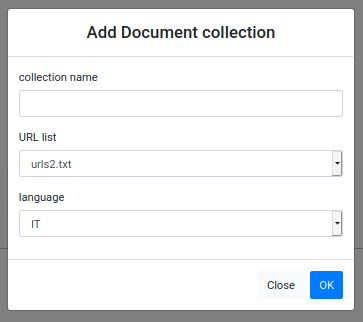
\includegraphics[width=.6\linewidth]{img/indexing2}
         \caption{popup for defining  document collections}
         \label{fig:indexingB}
     \end{subfigure}
   %  \hfill

\end{figure}

\subsection{Setting up an experiment}

The U.I. for experiment setup allows to define the details of an experiment to be carried out. This step involves creating
test groups with associated participants and document collections. Groups can be defined either manually or by using an
 uploaded configuration file. In both cases the test group configuration can later be edited manually. 
The interface allows to link each group to a set of previously indexed document collections. 
\textbf{Figure ~\ref{fig:setup}} shows this U.I.

\begin{figure} [h]
\centering
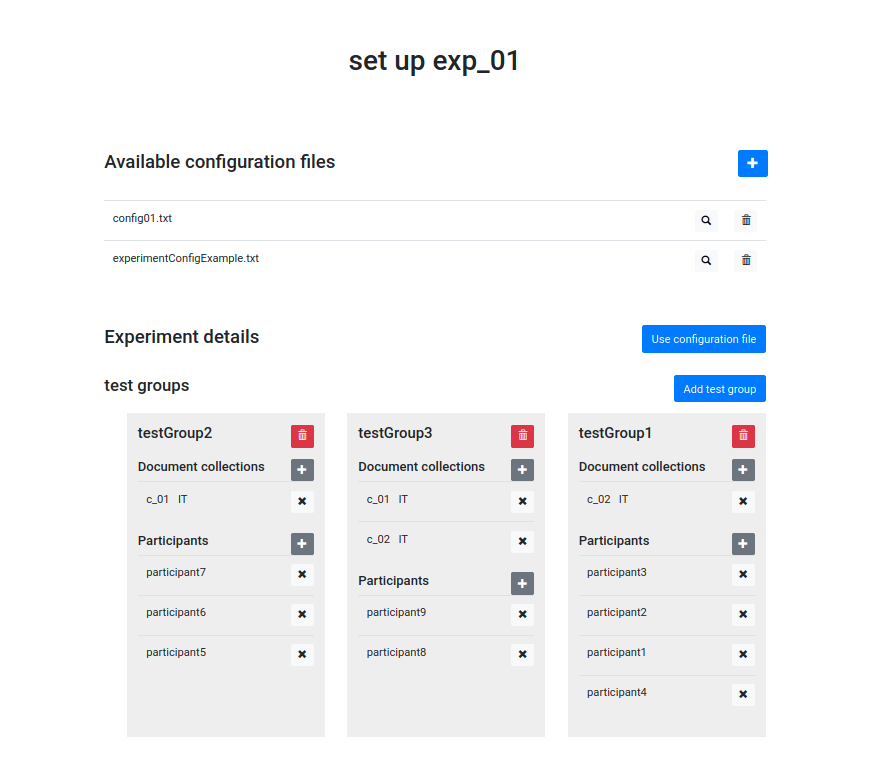
\includegraphics[width=0.8\textwidth]{img/setup}
\caption{U.I. for experiment setup}
\label{fig:setup}
\end{figure}

\subsection{Running an experiment}

The U.I. for experiment execution inccludes a start/stop/reset button, a timer, and a tabular display 
showing the current participant activities. Clicking the start button starts the timer, enables the participants to log in and
initiates the data collection process. While the experiment is running, all queries and click carried out by the
participants are stored as database records including a timestamp, user id, group id, and query/document related data.
The details of the data collection process are described in section xxx \TODO{link actual section}.
When the stop button is clicked the participants are logged out and all transient data is saved to the database.
after the experiment is complete the related evaluation page becomes available.
In case something goes wrong, the experiment can be reset. This causes all query and click data to be deleted, while the
experiments configuration is preserved.
\textbf{Figure ~\ref{fig:run}} shows this U.I.

\begin{figure} [h]
\centering
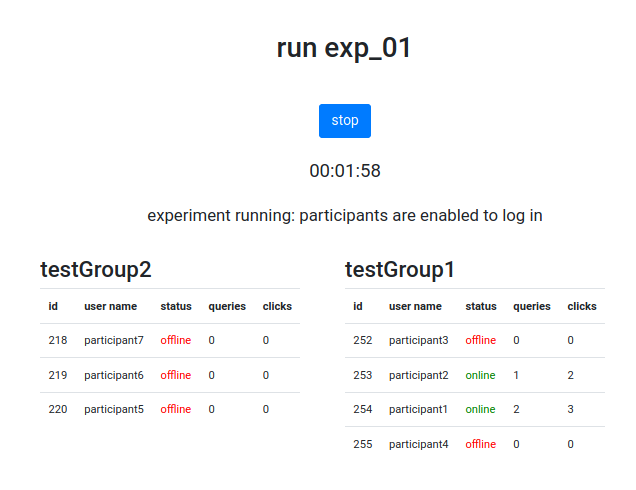
\includegraphics[width=0.6\textwidth]{img/run}
\caption{U.I. for experiment execution}
\label{fig:run}
\end{figure}

\subsection{Search user interface available to participants}

The interface available to the participants looks similar to the main page of most known search engines. It simply
includes a search text bar and a button for entering queries, and displays the results as a list of
links accompanied by short summaries (snippets) with highlighted query terms. 
\textbf{Figure ~\ref{fig:searchUi}} shows the U.I. after a query has been entered.

\begin{figure} [h]
\centering
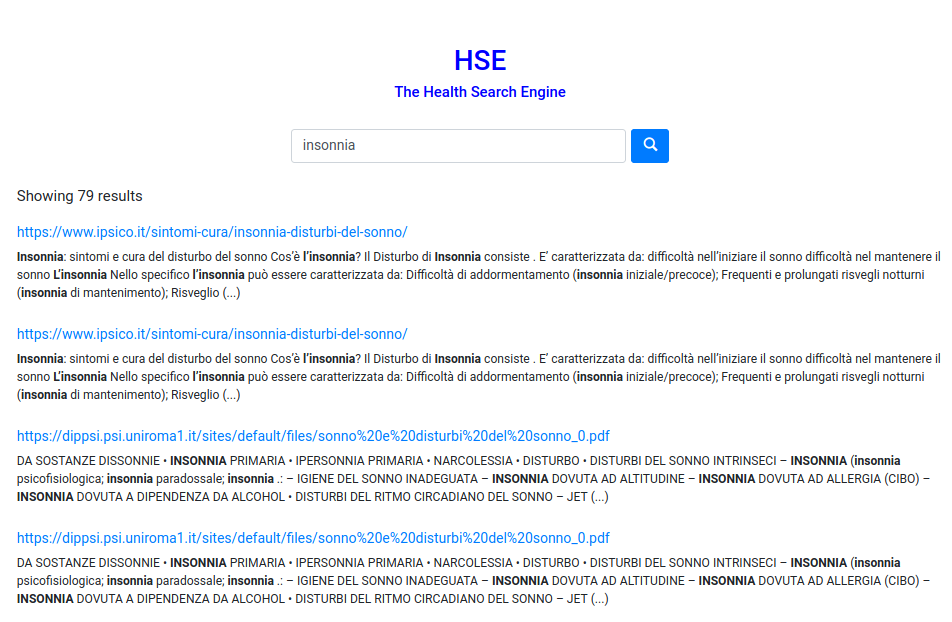
\includegraphics[width=0.8\textwidth]{img/searchUi}
\caption{User interface available to participants}
\label{fig:searchUi}
\end{figure}




%%%%%%%%%%%%%%%%%%%%%%%%%
\section{Implementation details} \label{implementation}
%%%%%%%%%%%%%%%%%%%%%%%%%

\TODO{}


%%%%%%%%%%%%%%%%%%%%%%%%%
\section{Quality assessment and evaluation} \label{evaluation}
%%%%%%%%%%%%%%%%%%%%%%%%%

\TODO{}

%%%%%%%%%%%%%%%%%%%%%%%%%
\section{Conclusions} \label{conclusions}
%%%%%%%%%%%%%%%%%%%%%%%%%

\TODO{}

%%%%%%%%%%%%%%%%%%%%%%%%%
\section{Future work} \label{futureWork}
%%%%%%%%%%%%%%%%%%%%%%%%%

\TODO{}


%%%%%

\newpage

\bibliographystyle{abbrv}
\bibliography{references}

\end{document}








